%%%%%%%%%%%%%%%%%%%%%%%%%%%%%%%%%%%%%%%%%%%%%%%%%%%%%%%%%%%%%%%%%%%%%%%%%%%%%
% Баталов Семен, 2021                                                       %
%%%%%%%%%%%%%%%%%%%%%%%%%%%%%%%%%%%%%%%%%%%%%%%%%%%%%%%%%%%%%%%%%%%%%%%%%%%%%

\documentclass[12pt, a4paper]{article}
\usepackage[left=2.5cm, right=2.5cm, top=2.5cm, bottom=2.5cm]{geometry}
\usepackage[utf8]{inputenc}
\usepackage{graphicx}
\graphicspath{{./pictures/}}
\usepackage[english, russian]{babel}
\usepackage{indentfirst}
\usepackage{misccorr}
\usepackage{amsmath}

\title{Регрессионный анализ точек на плоскости}
\author{Баталов Семен}
\date{25.02.2021}

\begin{document}
    
    \sloppy
    
    \maketitle
    
    \section{Постановка задачи}
    
    Требуется написать программу, которая для некоторых данных на плоскости 
    подбирает оптимальную регрессионную модель, и проверить корректность ее 
    работы на известных примерах.
    
    \section{Регрессионный анализ}
    
    Регрессионный анализ~--~набор статистических методов исследования 
    влияния одной или нескольких независимых переменных на зависимую 
    переменную. Наиболее распространенный вид регрессионного 
    анализа~--~линейная регрессия, когда находят линейную функцию, которая, 
    согласно определённым математическим критериям, наиболее соответствует 
    данным. Например, в методе наименьших квадратов вычисляется прямая (или 
    гиперплоскость), сумма квадратов между которой и данными минимальна.
    
    \begin{equation}
        y(w, x) = w_{0} + w_{1} \cdot x
        \label{eq21}
    \end{equation}
    
    Мы будем рассматривать одномерную задачу и использовать не только 
    линейные функции (\ref{eq21}), но и полиномы (\ref{eq22}), то есть будем 
    решать задачу не только линейной, но и полиномиальной регрессии.
    
    \begin{equation}
        y(w, x) = w_{0} + w_{1} \cdot x + w_{2} \cdot x^{2} + \cdots + w_{n} 
        \cdot x^{n}
        \label{eq22}
    \end{equation}
    
    Основная идея состоит в том, чтобы взять $x^{i}$ за новые переменные 
    $z_{i}$. Тем самым задача сведется к линейному (многомерному) случаю 
    (\ref{eq13}).
    
    \begin{equation}
        y(w, z) = w_{0} + w_{1} \cdot z_{1} + w_{2} \cdot z_{2} + \cdots + 
        w_{n} \cdot z_{n}
        \label{eq13}
    \end{equation}
    
    \section{Инструменты}
    
    Языком разработки является <<\textbf{Python}>>. Для работы с алгоритмом 
    линейной регрессии используется библиотека 
    <<\textbf{sklearn.linear\_model}>>. Для преобразования полинома в 
    функцию многих переменных используется 
    <<\textbf{sklearn.preprocessing}>>. Математическое обеспечение~--~
    библиотека <<\textbf{numpy}>>. Подробнее о программе можно узнать в 
    папке <<\textbf{source}>> проекта.
    
    \section{Примеры}
    
    Будем решать задачу регрессии для набора точек, который сформирован на 
    плоскости с помощью нормального распределения (\ref{eq41}).
    
    \begin{equation}
        f(x) = \frac{1}{\sigma \sqrt{2\pi}} \cdot exp\Big(-\frac{(x - 
            \mu)^{2}}{2\sigma^{2}}\Big)
        \label{eq41}
    \end{equation}
    
    Набор сотавлен так, чтобы приближать некоторую заранее известную 
    функцию. Зная это, можно оценить корректность работы программы. 
    Специфической особенностью программы можно считать необходимость 
    указания стартовой степени приближающего полинома. Алгоритм устроен так, 
    что он будет перебирать степени полиномов (начиная со стартовой) до тех 
    пор, пока точность очередной модели не будет <<сильно>> отличаться от 
    точности предыдущей. Под <<точностью>> подразумевается коэффициент 
    детерминации $R^{2}$.
    
    \subsection{$y(x) = x^{3}$}
    
    Рассматриваем промежуток $x \in (-3, 3)$. Стартовая степень полинома 
    $deg(p) = 2$. На рис.~\ref{image41}.1 изображен результат работы 
    программы.
    
    \begin{figure}[h!]
        \center
        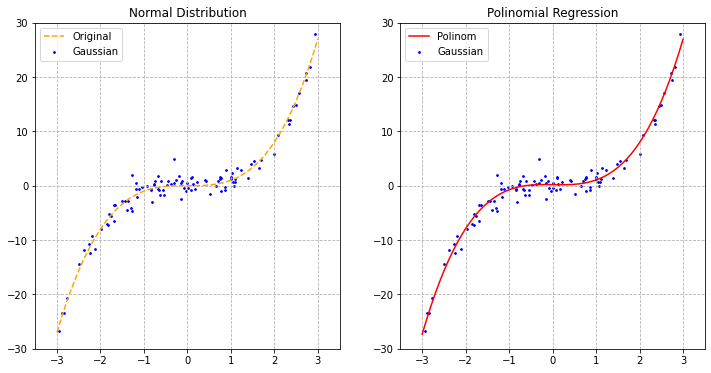
\includegraphics[width = 14cm]{f1.png}
        \label{image41}
        \caption{Регрессионная модель для $y(x) = x^{3}$; $deg(p_{opt}) = 
            3$.}
    \end{figure}
    
    Для данной задачи степень оптимального полинома $deg(p_{opt}) = 3$. 
    Коэффициент детерминации $R^{2} = 0.976$.
    
    \subsection{$y(x) = 5 \cdot x^{2}$}
    
    Рассматриваем промежуток $x \in (-3, 3)$. Стартовая степень полинома 
    $deg(p) = 2$. На рис.~\ref{image42}.2 изображен результат работы 
    программы.
    
    \begin{figure}[h!]
        \center
        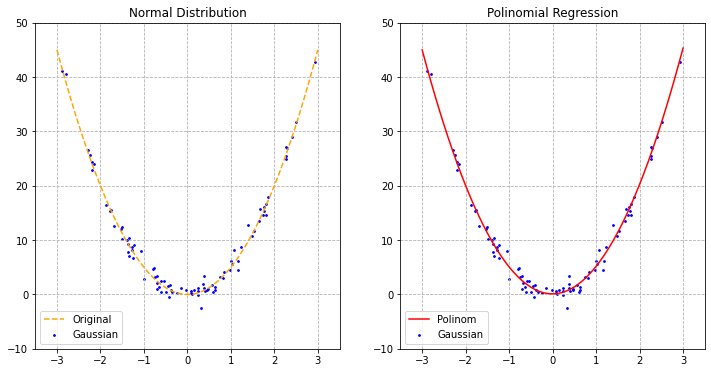
\includegraphics[width = 14cm]{f2.png}
        \label{image42}
        \caption{Регрессионная модель для $y(x) = 5 \cdot x^{2}$; 
            $deg(p_{opt}) = 2$.}
    \end{figure}
    
    Для данной задачи степень оптимального полинома $deg(p_{opt}) = 2$. 
    Коэффициент детерминации $R^{2} = 0.988$.
    
    \subsection{$y(x) = 0.7 \cdot x + 2$}
    
    В данном случае рассмотрим частный случай полиномиальной 
    регрессии~--~линейную регрессию. Рассматриваем промежуток $x \in (1, 
    10)$. Стартовая степень полинома $deg(p) = 1$. На рис.~\ref{image43}.3 
    изображен результат работы программы.
    
    \begin{figure}[h!]
        \center
        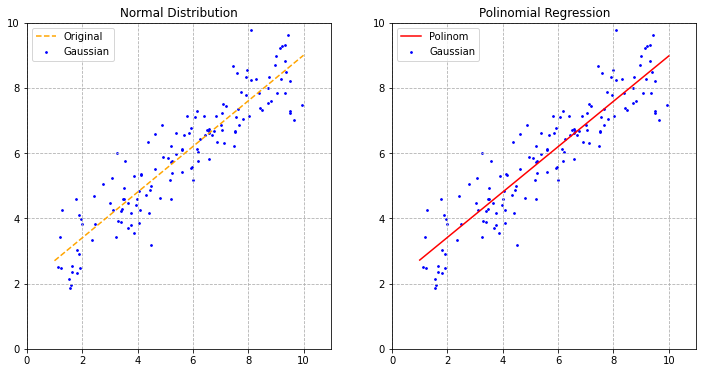
\includegraphics[width = 14cm]{f3.png}
        \label{image43}
        \caption{Регрессионная модель для $y(x) = 0.7 \cdot x + 2$; 
            $deg(p_{opt}) = 1$.}
    \end{figure}
    
    Для данной задачи степень оптимального полинома $deg(p_{opt}) = 1$. 
    Коэффициент детерминации $R^{2} = 0.837$.
    
    \subsection{$y(x) = sin(x)$}
    
    Рассматриваем промежуток $x \in (-3, 3)$. Стартовая степень полинома 
    $deg(p) = 1$. На рис.~\ref{image44}.4 изображен результат работы 
    программы.
    
    \begin{figure}[h!]
        \center
        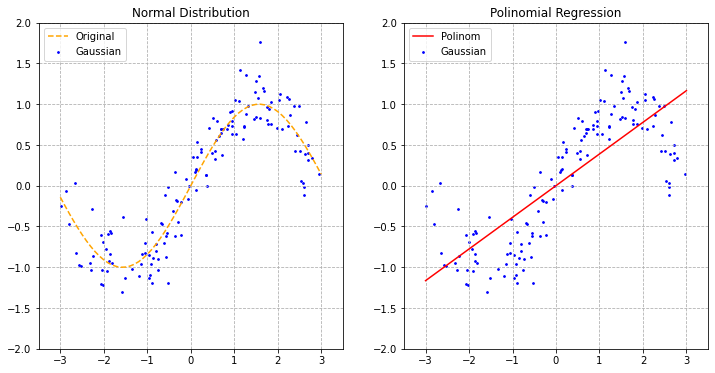
\includegraphics[width = 14cm]{f4_1.png}
        \label{image44}
        \caption{Регрессионная модель для $y(x) = sin(x)$; $deg(p_{opt}) = 
            1$.}
    \end{figure}
    
    При установленной точности степень оптимального полинома $deg(p_{opt}) = 
    1$. Коэффициент детерминации $R^{2} = 0.621$.
    
    Теперь потребуем большей точности (начальные условия те же). Результат 
    работы программы изменится (рис.~\ref{image45}.5).
    
    \begin{figure}[h!]
        \center
        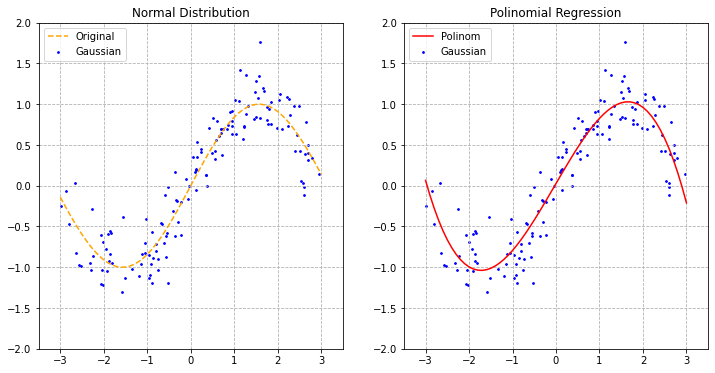
\includegraphics[width = 14cm]{f4_2.png}
        \label{image45}
        \caption{Регрессионная модель для $y(x) = sin(x)$; $deg(p_{opt}) = 
            3$.}
    \end{figure}
    
    При установленной точности степень оптимального полинома $deg(p_{opt}) = 
    3$. Коэффициент детерминации $R^{2} = 0.881$.
    
    Вновь потребуем большей точности (начальные условия те же). Результат 
    работы программы изменится (рис.~\ref{image46}.6).
    
    \begin{figure}[h!]
        \center
        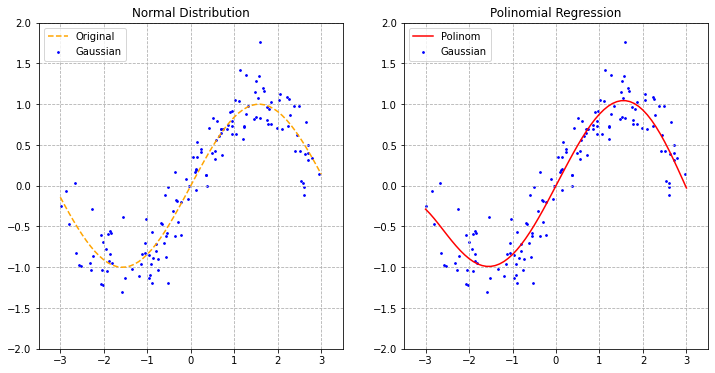
\includegraphics[width = 14cm]{f4_3.png}
        \label{image46}
        \caption{Регрессионная модель для $y(x) = sin(x)$; $deg(p_{opt}) = 
            5$.}
    \end{figure}
    
    При вновь установленной точности степень оптимального полинома 
    $deg(p_{opt}) = 5$. Коэффициент детерминации $R^{2} = 0.888$.
    
    \subsection{$y(x) = exp(x)$}
    
    Рассматриваем промежуток $x \in (-3, 5)$. Стартовая степень полинома 
    $deg(p) = 1$. На рис.~\ref{image47}.7 изображен результат работы 
    программы.
    
    \begin{figure}[h!]
        \center
        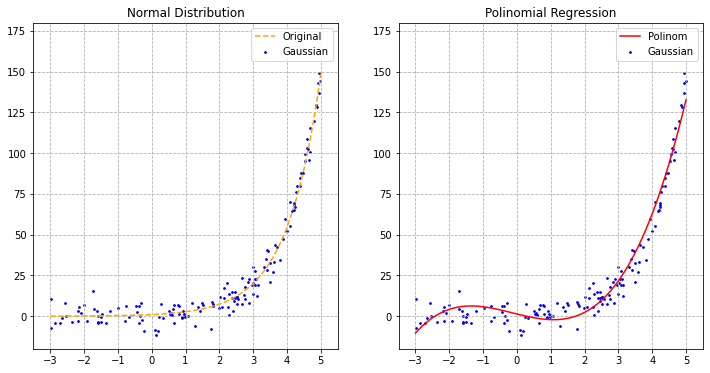
\includegraphics[width = 14cm]{f5_1.png}
        \label{image47}
        \caption{Регрессионная модель для $y(x) = exp(x)$; $deg(p_{opt}) = 
            3$.}
    \end{figure}
    
    При установленной точности степень оптимального полинома $deg(p_{opt}) = 
    3$. Коэффициент детерминации $R^{2} = 0.965$.
    
    Теперь потребуем большей точности (начальные условия те же). Результат 
    работы программы изменится (рис.~\ref{image48}.8).
    
    \begin{figure}[h!]
        \center
        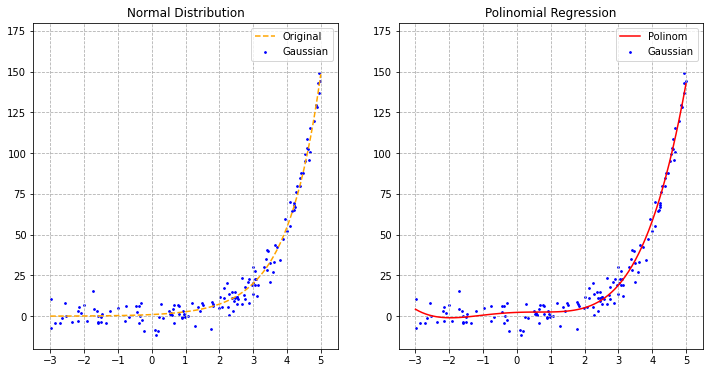
\includegraphics[width = 14cm]{f5_2.png}
        \label{image48}
        \caption{Регрессионная модель для $y(x) = exp(x)$; $deg(p_{opt}) = 
            4$.}
    \end{figure}
    
    При установленной точности степень оптимального полинома $deg(p_{opt}) = 
    4$. Коэффициент детерминации $R^{2} = 0.977$.
    
    Вновь потребуем большей точности (начальные условия те же). Результат 
    работы программы изменится (рис.~\ref{image49}.9).
    
    \begin{figure}[h!]
        \center
        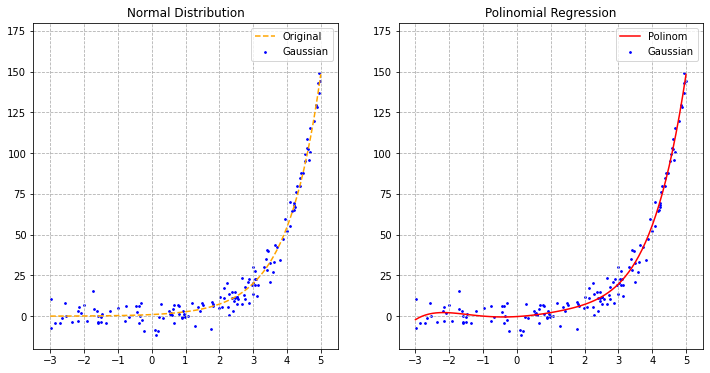
\includegraphics[width = 14cm]{f5_3.png}
        \label{image49}
        \caption{Регрессионная модель для $y(x) = exp(x)$; $deg(p_{opt}) = 
            5$.}
    \end{figure}
    
    При вновь установленной точности степень оптимального полинома 
    $deg(p_{opt}) = 5$. Коэффициент детерминации $R^{2} = 0.981$.
    
    \section{Выводы}
    
    В итоге составили программу, которая автоматически подбирает оптимальную 
    регрессионную (полиномиальную) модель. Проверили ее работоспособность 
    (используя нормальное распределенние точек на плоскости) на известных 
    примерах функций, убедились, что она работает корректно. Более того, 
    выяснили, что, меняя входные параметры алгоритма, можно получать разные 
    приближающие полиномы и влиять на точность регрессионной модели 
    (коэффициент детерминации).
    
\end{document}